
% Template for Elsevier CRC journal article
% version 1.0 dated 13 October 2009

% This file (c) 2009 Elsevier Ltd.  Modifications may be freely made,
% provided the edited file is saved under a different name

% This file contains modifications for Procedia Computer Science

%%%%%%%%%%%%%%%%%%%%%%%%%%%%%%%%%%%%%%%%%%%%%%%%%%%%%%%%%%%%%%%%%%%%%%%%%%

%% This template uses the elsarticle.cls document class and the extension package ecrc.sty
%% For full documentation on usage of elsarticle.cls, consult the documentation "elsdoc.pdf"
%% Further resources available at http://www.elsevier.com/latex

%%%%%%%%%%%%%%%%%%%%%%%%%%%%%%%%%%%%%%%%%%%%%%%%%%%%%%%%%%%%%%%%%%%%%%%%%%

%% The '1p' and 'times' class options of elsarticle are used for Elsevier CRC
\documentclass[1p,times]{elsarticle}

%% The `ecrc' package must be called to make the CRC functionality available
\usepackage{ecrc}

%% The ecrc package defines commands needed for running heads and logos.
%% For running heads, you can set the journal name, the volume, the starting page and the authors

%% set the volume if you know. Otherwise `00'
\volume{00}

%% set the starting page if not 1
\firstpage{1}

%% Give the name of the journal
\journalname{Procedia Computer Science}

%% Give the author list to appear in the running head
%% Example \runauth{C.V. Radhakrishnan et al.}
\runauth{V. Kuznetsov, D. Evans, S. Metson}

%% The choice of journal logo is determined by the \jid and \jnltitlelogo commands.
%% A user-supplied logo with the name <\jid>logo.pdf will be inserted if present.
%% e.g. if \jid{yspmi} the system will look for a file yspmilogo.pdf
%% Otherwise the content of \jnltitlelogo will be set between horizontal lines as a default logo

%% Give the abbreviation of the Journal.
\jid{procs}

%% Give a short journal name for the dummy logo (if needed)
\jnltitlelogo{Procedia Computer Science}

%% Hereafter the template follows `elsarticle'.
%% For more details see the existing template files elsarticle-template-harv.tex and elsarticle-template-num.tex.

%% Elsevier CRC generally uses a numbered reference style
%% For this, the conventions of elsarticle-template-num.tex should be followed (included below)
%% If using BibTeX, use the style file elsarticle-num.bst

%% End of ecrc-specific commands
%%%%%%%%%%%%%%%%%%%%%%%%%%%%%%%%%%%%%%%%%%%%%%%%%%%%%%%%%%%%%%%%%%%%%%%%%%

%% The amssymb package provides various useful mathematical symbols
\usepackage{amssymb}
%% The amsthm package provides extended theorem environments
%% \usepackage{amsthm}

%% The lineno packages adds line numbers. Start line numbering with
%% \begin{linenumbers}, end it with \end{linenumbers}. Or switch it on
%% for the whole article with \linenumbers after \end{frontmatter}.
%% \usepackage{lineno}

%% natbib.sty is loaded by default. However, natbib options can be
%% provided with \biboptions{...} command. Following options are
%% valid:

%%   round  -  round parentheses are used (default)
%%   square -  square brackets are used   [option]
%%   curly  -  curly braces are used      {option}
%%   angle  -  angle brackets are used    <option>
%%   semicolon  -  multiple citations separated by semi-colon
%%   colon  - same as semicolon, an earlier confusion
%%   comma  -  separated by comma
%%   numbers-  selects numerical citations
%%   super  -  numerical citations as superscripts
%%   sort   -  sorts multiple citations according to order in ref. list
%%   sort&compress   -  like sort, but also compresses numerical citations
%%   compress - compresses without sorting
%%
%% \biboptions{comma,round}

% \biboptions{}

% if you have landscape tables
\usepackage[figuresright]{rotating}

% put your own definitions here:
%   \newcommand{\cZ}{\cal{Z}}
%   \newtheorem{def}{Definition}[section]
%   ...

% add words to TeX's hyphenation exception list
%\hyphenation{author another created financial paper re-commend-ed Post-Script}

% mdwlist allows you to create e.g. bulleted lists without extra line spacing
\usepackage{mdwlist}

% declarations for front matter

\begin{document}

\begin{frontmatter}

%% Title, authors and addresses

%% use the tnoteref command within \title for footnotes;
%% use the tnotetext command for the associated footnote;
%% use the fnref command within \author or \address for footnotes;
%% use the fntext command for the associated footnote;
%% use the corref command within \author for corresponding author footnotes;
%% use the cortext command for the associated footnote;
%% use the ead command for the email address,
%% and the form \ead[url] for the home page:
%%
%% \title{Title\tnoteref{label1}}
%% \tnotetext[label1]{}
%% \author{Name\corref{cor1}\fnref{label2}}
%% \ead{email address}
%% \ead[url]{home page}
%% \fntext[label2]{}
%% \cortext[cor1]{}
%% \address{Address\fnref{label3}}
%% \fntext[label3]{}

\dochead{International Conference on Computational Science, ICCS 2010}
%% Use \dochead if there is an article header, e.g. \dochead{Short communication}

\title{The CMS Data Aggregation System}

%% use optional labels to link authors explicitly to addresses:
%% \author[label1,label2]{<author name>}
%% \address[label1]{<address>}
%% \address[label2]{<address>}

%\author[vkuznet]{Valentin Kuznetsov\corref{cor1}}
\author[vkuznet]{Valentin Kuznetsov}
\address[vkuznet]{Cornell University, Ithaca, New York, USA}
%\ead{vkuznet@gmail.com}

\author[evans]{Dave Evans}
\address[evans]{Fermilab, Batavia, Illinois, USA}
%\ead{evansde@fnal.gov}

\author[metson]{Simon Metson}
\address[metson]{Bristol University, Bristol, UK}
%\ead{s.metson@bristol.ac.uk}

%\cortext[cor1]{Corresponding author}

\begin{abstract}
Meta-data plays a significant role in large modern enterprises, 
research experiments and digital libraries where it comes from many different 
sources and is distributed in a variety of digital formats. 
It is organized and managed by constantly evolving software using 
both relational and non-relational data sources. Even though we can apply
an information retrieval approach to non-relational data sources,
we can't do so for relational ones, where information is accessed via
a pre-established set of data-services.

Here we discuss a new data aggregation system which consumes, 
indexes and delivers information from different relational and 
non-relational data sources to answer cross data-service queries 
and explore meta-data associated with petabytes of experimental data. 
We combine the simplicity of keyword-based search with the precision of RDMS
under the new system. The aggregated information is collected from various sources,
allowing end-users to place dynamic queries, get precise answers and 
trigger information retrieval on demand. Based on the use cases of the CMS experiment, 
we have performed a set of detailed, large scale tests the results of which 
we present in this paper.
\end{abstract}

\begin{keyword}
%% keywords here, in the form: keyword \sep keyword
Meta-data\sep data aggregation\sep information discovery\sep HEP.

%% PACS codes here, in the form: \PACS code \sep code

%% MSC codes here, in the form: \MSC code \sep code
%% or \MSC[2008] code \sep code (2000 is the default)
\end{keyword}

\end{frontmatter}

%%
%% Start line numbering here if you want
%%
% \linenumbers

%% main text
\section{Introduction}
The European Organization for Nuclear Research, known as CERN, plays a leading
role in fundamental studies of physics. It is also known as a place where
many innovations in the area of computer science were developed, e.g. The World Wide Web.
Today, the Large Hadron Collider (LHC) at CERN is marking a new era of High Energy
Physics (HEP), promising to deliver a few PB of data each year. 
At this scale the ``information discovery'' within a heterogeneous, distributed 
environment becomes a key ingredient of successful data analysis.
The data and associated meta-data are produced in variety of forms and digital formats.
They are stored and retrieved from relational and non-relational data-sources, such as 
RDMS systems, document oriented databases, blogs, twikies, file systems,
customized applications, etc. Working in such an environment requires a lot 
of expertise and demands a straightforward, simple
way to look-up the desired information.
A well-known solutions, e.g. data-services, are tighten to a specific data 
sources and end-users are left with a manual task to bookkeep and 
relate information from them.

Here we present our work on Data Aggregation System (DAS) which provides
ability to search and aggregate information across different 
data-services. While designed for CMS High-Energy Physics 
experiment at LHC, the strategies and technology could be
used elsewhere. 

The rest of this paper is organized as follows. 
In section \ref{RelatedWork} we discuss related work in a domain of 
keyword search over relational data sources.
Section \ref{DataModel} breifly describes the Compact Muon Solenoid (CMS) experiment 
and its data model. In section \ref{DAS} we present the architecture 
of the DAS system, including discussion of its
various components. Finally, our results are summarized in section \ref{Results}.

\section{Related Work\label{RelatedWork}}
Even though the idea of keyword queries over the relational database
is not knew it is still under discussion in computer science domain.
A few alternative solutions have been proposed to address this issue
in last several years. In \cite{DBXplorer} the conjunctive keyword queries,
i.e. retrieval of documents that contain all query keywords, has
been discussed. It requires that all keywords are matched in a row from a
single table or joined tables. Authors of \cite{QueryAnswer} make a step forward
and have evaluated information around matched values. The results were presented as
customized templates to end-users. 
These and other related works, (see \cite{DBXplorer, QueryAnswer} 
for more references), are based on an approach that builds some 
kind of the graph over the underlying 
database and generates a new database out of the source database to perform the work.
The proximity of the results in those techniques are mostly confined to a 
text-based values stored in a database, since the usage of numerical ones 
is mostly useless without knowledge of the context of the input value. 
For example, typing a value 100 in the search input field can lead to 
plenty of inappropriate matches, e.g. row ids. In order to be
answered correctly it requires an additional keyword to clarify its meaning, 
which should be matched with particular entity (table.column) in the 
underlying database. Therefore the logical questions, e.g.
{\it find me the total number of files whose size more then 20 but less then 
100} are hard to answer precisely using approaches outlined in \cite{DBXplorer, QueryAnswer}, 
while it can be easily accomplished using SQL. 

To address these limitations a keyword-based query language was introduced in \cite{DBS-QL}.
It used a set of pre-defined keys mapped to an underlying schema and shortest path
algorithm which employed foreign key constraints to build SQL queries. As a result
the question
{\it I'm looking for files who contain data taken on certain date and located at
particular site} was represented as simply as \cite{DBS-QL}
\begin{verbatim}
find file where date 2009-01-02 11:59 CET and site = T2
\end{verbatim}
without specifying any relational details.
This solution represents a common use case in the HEP community and provides
an intuitive mapping between the mental model of the end-users and 
the underlying database schema.

At the same time the data aggregation is commonly addressed in the context of
federated databases, see for example \cite{FedDB}. The data from different 
RDMS systems are stored into the federated DB where SQL queries can be used to 
search desired data. Apart from many internal obstacles, such as
schema, domain and naming conflicts, it is external issues that are often
a large barrier within a distributed, heterogeneous environment where
different security policies are in place. At the end the usage of SQL and/or
any other Query Language is required to search for data.

To avoid these limitations we resolved to build a keyword-search based system around
existing data-services whose nature and access policies are in place and well understood.
The key ingredients were the setup of the mapping and analytics services which provided
the necessary glue across existing API/notations and user queries. This approach 
allows us to perform dynamic data aggregation across various data-services, achieve
precise answers using keyword-based queries
and organize information retrieval on demand.

\section{CMS data model\label{DataModel}}
The Compact Muon Solenoid, (CMS) \cite{CMS} 
is one of the two general purpose particle physics detectors built on 
the Large Hadron Collider (LHC) at CERN in Switzerland and France. 
The experiment is designed to explore the frontiers of physics and provide physicists
with the ability to look at the conditions presented in the early stage of our Universe.
More then 3000 physicists from 183 institutions representing 38 countries 
are involved in the design, construction and maintenance of the experiment.

The CMS distributed computing and data model \cite{CMSDataModel} 
is designed to process and efficiently manage the few PBs of data expected each year
during normal operation of the LHC. The computing resources available to the CMS
collaboration are geographically distributed, 
interconnected via high throughput networks and operated by means 
of various Grid software infrastructure. The model is designed to
incorporate a broad variety of both mass data storage and data processing
resources into a single coherent system. CMS uses
multi-Tiered model, where specific tasks related to data taking such as
processing, archival and distribution, are assigned to each tier based
on the CMS data model. For example, the Tier-0 center at CERN is responsible
for archiving the data coming out from the detector, prompt first pass reconstruction
and data distribution to Tier-1 centers, located around the world.
The Tier-1 centers provide archival storage and CPU power for high
priority selection and re-reconstructions jobs and distribution points
to the Tier 2 resources.
The Tier-2 centers are dedicated for user analysis tasks and production of simulated data.

A broad variety of data-services have been designed and developed to
maintain detector and production operations, including detector
conditions databases, data bookkeeping services,
data transfer and job monitoring tasks. While the majority of these
services are located at CERN, they need to be accessed remotely, and
combined with other distributed services.

Once such a conglomerate of data-services start operating the obvious
question arises: how do we find the desired information across multiple data-services
in our distributed environment? Even though the individual data-services were designed
to answer specific questions about the data they serve, the ability to search and relate
information among them remains a tedious human task. The growing amount of information
and desire to make cross-service queries led us to design and develop the new
Data Aggregation System.

\section{Data Aggregation System\label{DAS}}
The goal of the Data Aggregation System (DAS) was to fetch and aggregate meta-data 
on demand from existing CMS data-services under one umbrella by using their APIs, 
security policies, etc. In contrast, the approaches
discussed in \cite{DBXplorer, QueryAnswer, FedDB}
enforce a publication step of data into a dedicated database 
or central repository \cite{iRODS}. Therefore, quite often it was required
that data should be converted into common data structure/format in order to enable
aggregation, see \cite{OpenArchive}. In DAS the data are provided
by existing data-services and infrastructure, whose implementation,
data representation and security policies are left intact. Consequently,
DAS does not require a data preservation and transaction capabilities. 
Instead DAS can be treated as proxy or caching layer where information 
retrieval and aggregation are triggered dynamically by user queries. 
Below we discuss in details the DAS architecture.

\subsection{DAS architecture}
The design of the DAS system was based on previous studies of CMS Data 
Bookkeeping System (DBS) \cite{DBS, DBS07}. The DBS Data Discovery service
\cite{DD} was based on DBS Query Language (DBS-QL) \cite{DBS-QL}. It provided
a syntax similar to SQL, without specific knowledge of the underlying DB schema.
Quick adoption and wide usage of DBS-QL in CMS gave us confidence in the chosen approach 
and provided a basis for building the DAS system.

As was pointed out in \cite{Arms} the mixed content and 
mixed meta-data and meta-data consistency 
of the underlying services needs to be carefully
considered in the design of the system if it is to be a successful information 
discovery service.
Starting from this ground we are designed the DAS system as an
additional layer on top of the existing data-services
within CMS computing infrastructure by imposing the following set of requirements:
support a keyword based search queries with ability to use conditional operators;
use existing heterogeneous software environment and distributed nature of the data-services;
preserve access rules and security policies of individual data-services;
retrieve data on demand and aggregate them if necessary across
multiple data-services;
be transparent to data-services implementation and their data formats.
%\begin{itemize}
%\item support a keyword based search queries with ability to use conditional operators;
%\item use existing heterogeneous software environment and distributed nature of the data-services;
%\item preserve access rules and security policies of individual data-services;
%\item retrieve data on demand and aggregate them if necessary across
%multiple data-services;
%\item be transparent to data-services implementation and their data formats;
%\end{itemize}
\begin{figure}[htb]
\centering
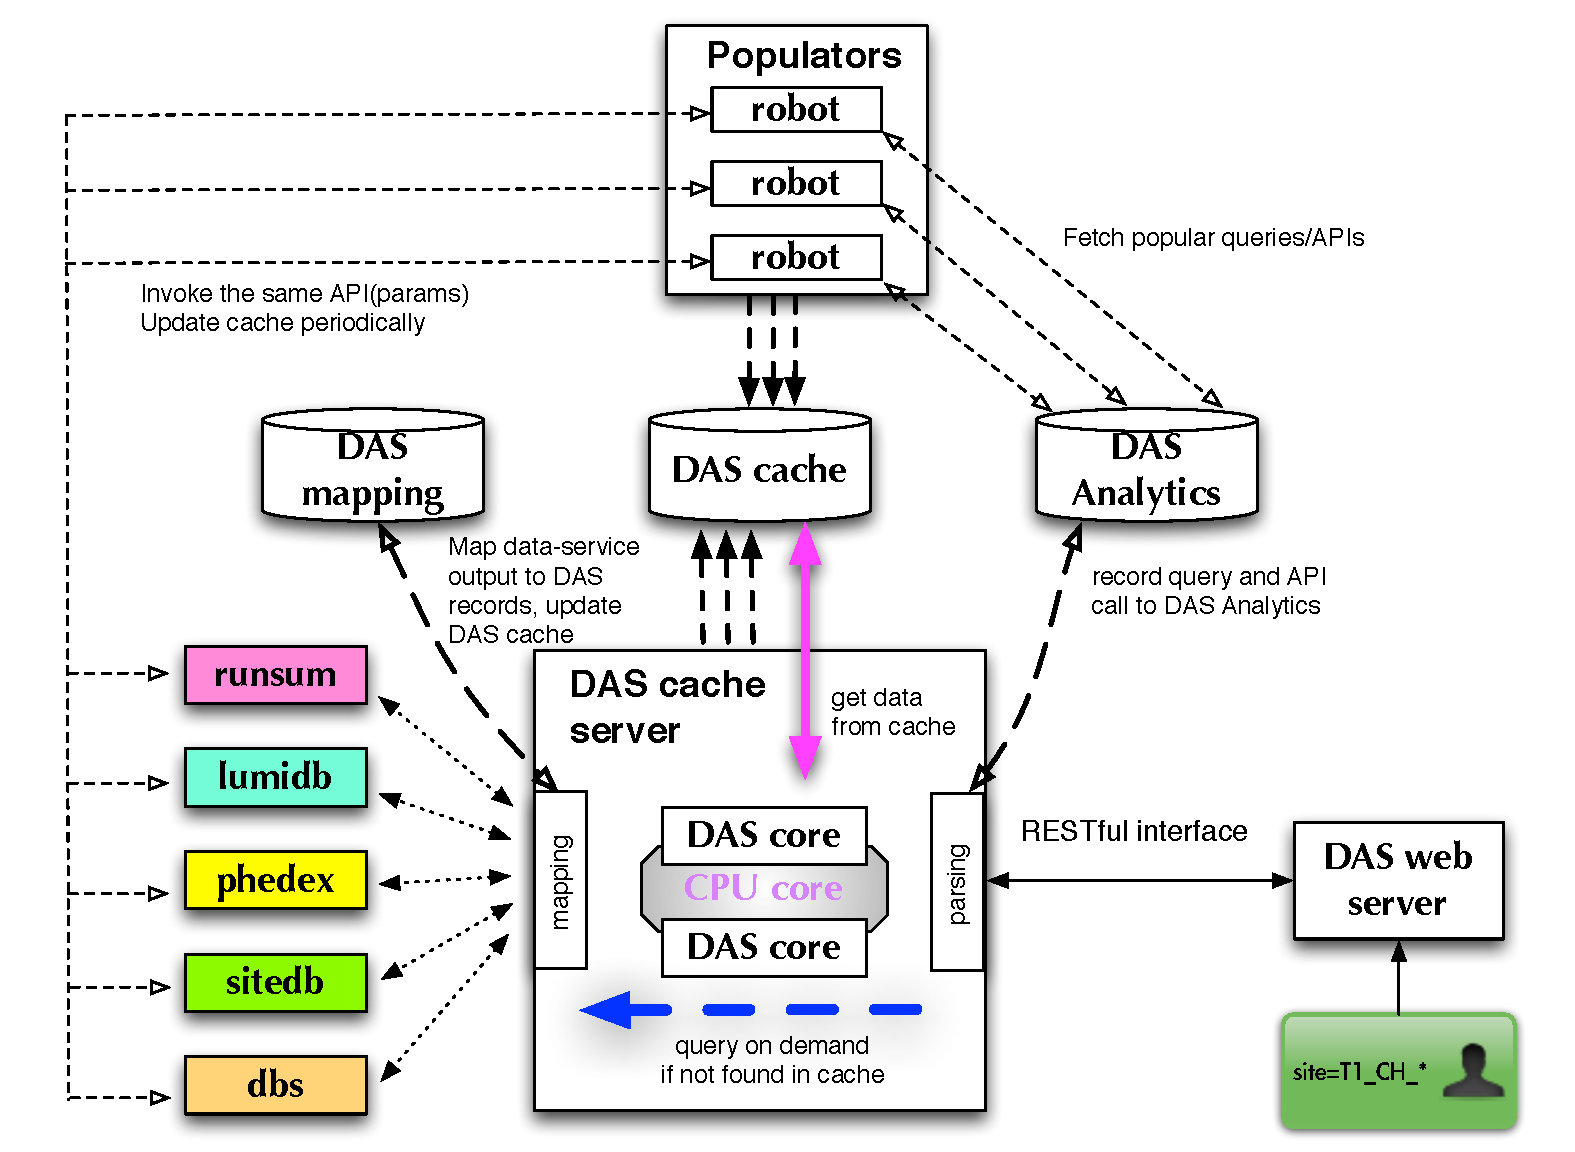
\includegraphics[width=90mm]{DAS_Cache_and_Analytics.pdf}
\caption{
The DAS architecture diagram. It consists of cache server,
analytics, mapping and cache databases. The data in a cache can be shared
across multiple queries. The information retrieval is triggered
on demand basis by invoking appropriate data-service APIs. The
optional DAS robots (Unix daemons) can be used to pre-fetch
the most popular query requests. The solid, dashed and dotted lines 
represent outer, inner and optional process communications between
different DAS components, respectively.
}
\label{DAS_cache}
\end{figure}

\noindent
The choice of existing RDMS as DAS back-end(s) were ruled out for several reasons. 
For instance, we didn't require any transactions and data persistency in DAS;
a dynamically typing of stored meta-data objects was one of the requirements, etc.
Those arguments forced us to look for alternative IT solutions.
Through the careful analysis of available options, such as a file-based and in memory caches, 
key-value databases, documented-oriented databases we made our choice in favor 
of the last technology. Among them we evaluated CouchDB \cite{CouchDB} and 
MongoDB \cite{MongoDB}. Both systems are ``schema-less'' databases providing
arbitrary document structure storage, replication and fail-over features. 
We made our decision in favor of MongoDB, due to its support of dynamic queries, 
full indexes, including inner objects and embedded arrays,
and auto-sharding. Our preliminary benchmarks have shown that it can sustain
the desired load and size capable of handling our meta-data information. We used 
document-oriented database, MongoDB, as a back-end for three 
main DAS components: Mapping, Analytics and DAS cache databases, 
which will be discussed next. 

The DAS architecture is shown in Fig. \ref{DAS_cache}. It consists of
the core library with support of pluggable modules for data retrieval;
caching layer to store and aggregate results into DAS Cache and DAS merge
databases, respectively;
request service to handle user queries;
Mapping DB to keep information about data-service APIs, e.g.
notations and mapping to DAS keys;
Analytics DB for query analysis.

\subsection{DAS core\label{DAS_core}}
The DAS core library is responsible for data retrieval on demand. 
It has the following components: input query validator and parser,
query analyzer, workflow builder, execution engine and data-service 
plug-ins. The communication between client (web server or CLI) and 
DAS cache server is done via the REST \cite{REST} interface. 
Each input query is recorded into the Analytics DB for further 
analysis, and is decomposed into a set of conditions and/or selection keys.
First the results are looked up in a cache and delivered to the requester
if superset of input conditions is found in analytics DB.\footnote{It is important
to note here that we didn't look-up results in a cache and rather
compared input query condition set to the records in analytics DB 
in order to understand if other API calls are covered the input request.}
Otherwise, the appropriate workflow, a set of API calls, is constructed
for the execution engine. It invoked the API calls via data-service
plug-ins and stored results into the cache. At this step we also
performed necessary data aggregation for records with similar key-value
pairs. The data-service plug-in implementations are similar and their 
logic is largely abstracted, apart from a few extensions such as specific
security modules for data-services accessible via private network.
Finally, the results are retrieved from the cache and delivered to the user. 

\subsection{DAS Mapping DB\label{MappingDB}}
The Mapping DB is used to track services known to DAS and how DAS should interact with them.
It collects
information about data-service APIs, translates API input/output
parameters into DAS keys and contains mapping between DAS records
and their UI representation.

On identifying API's that are accessible to DAS we store
their names, input parameters and associated DAS keys
into the Mapping DB. For example
\begin{verbatim}
{"system": "phedex", "format": "XML", "urn": "fileReplicas",
 "url": "http://a.b.com/phedex/datasvc/xml/prod/fileReplicas", 
 "params": {"node": "*", "block": "required", "se": "*"}, 
 "api2das": [{"pattern": "", "das_key": "file.block.name", 
    "api_param": "block"}, {"pattern": "re.compile('^T[0-3]_')", 
    "das_key": "site", "api_param": "node"}], 
 "daskeys": [{"map": "file.name", "key": "file", "pattern": ""}, 
             {"map": "file.block.name", "key": "block", "pattern": ""}]}
\end{verbatim}
represents DAS mapping record.
This record can be read as following:
the \verb+fileReplicas+ API (urn) provided by given url delivers data in
XML data format and belongs to \verb+phedex+ system.
It accepts \verb+node+, \verb+block+ and \verb+se+ input parameters, shown in \verb+params+ part
of the record. Each record has two maps: \verb+api2das+ for mapping api input parameters into
DAS keys and \verb+daskeys+ for mapping input DAS keys into DAS record access keys.


Therefore the Mapping DB identifies a set of pre-defined DAS keys, 
e.g. \verb+file, block+, etc., to be used by end-users in their queries.
Each key is mapped onto set of API calls, whose output is retrieved,
cached and aggregated as required. 

\subsection{DAS Analytics DB}
The DAS Analytics DB collects information on user requests against the system.
Each request that DAS handles is recorded.
The Analytics DB tracks: the users request; how DAS has mapped the request 
onto data service API's; the time taken by the remote data services to 
process the API calls.

By recording this information we can plan pre-fetch strategies for common queries,
identify issues in remote data services and cross check that DAS resolves requests
in a deterministic manner.

% Upon its
%decomposition into set of selection keys and conditions we also recorded
%API name and input parameters into the Analytics DB and 
%kept updating their counter information for repeated calls. 
%This allowed to keep track of frequency of API calls and establish 
%pre-fetch strategies for most common queries.

\subsection{DAS caching system}
The DAS caching system is used to dynamically fetch
and aggregate data upon user requests. It consits of
DAS cache and DAS merge independent databases. The former one is used to store
the raw results coming out from data-services, while the later contains aggregated
records. Each data record in DAS cache/merge DBs contains expiration timestamps 
provided either by data-service itself or based on default values during 
data-service registration.
We use the following algorithm (code snippets are written in Python \cite{Python}):
\begin{enumerate}[1.]
\item Decompose query into set of conditions (\verb+conds+) 
and selection keys (\verb+skeys+).
\item Check cache for query hash. If found, look-up results from the cache,
otherwise proceed to the next step.
\item Identify list of APIs which can serve requested data
\begin{verbatim}
apilist = [r for r in mapping_db(skeys, conds)]
\end{verbatim}
Here \verb+r+ represents a triplet \verb+url, api, args+ and 
\verb+mappind_db+ defines translation between input query and data-service
APIs which can delivery the data.
\item Iterate over APIs
\begin{verbatim}
for url, api, args in apilist:
    if  superset_in_analytics(api, args):
        continue
    for row in parser(get_data(url, api, args)):
        yield row
\end{verbatim}
Here \verb+superset_in_analytics+ checks if provided \verb+api, args+
are subset of already registered in Analytics DB api call(s). The 
\verb+get_data+ and \verb+parser+ are define methods to fetch and parse
data, respectively.
\item Perform aggregation by iterating over records from the previous step
\begin{verbatim}
if cache_has(daskey):
   existing_record = get_from_cache(daskey)
   merge(row, existing_record)
   insert_into_cache(row)
else:
   insert_into_cache(row)
\end{verbatim}
The \verb+daskey+
is a key which identifies the record defined in Mapping DB, e.g. \verb+file.name+
for \verb+file+ record.
We did use a bulk insert operations at this step to increase throughput. 
\item Get results from the cache
\end{enumerate}
%We also have an option to run independent set of daemons, DAS robots, who
%monitor Analytics DB for most popular requests and pre-fetch the most
%common data into the cache. 
We can also automate populating the cache by running an 
independent set of daemons, DAS robots, which monitor the 
Analytics DB for suitable requests (for example queries that are 
popular, periodic in nature or expensive) and pre-fetch data into the cache. 

\subsection{DAS queries}
All DAS queries are expressed in a free text-based form, either as a 
set of keywords or key-value pairs, where a pair can represent
condition, e.g. \verb+key > value+. We use a pre-defined set of keys registered 
in DAS to describe common entities of our data. For example, \verb+dataset+, 
\verb+file+, \verb+block+, \verb+run+, \verb+event+, etc. The choice of keys
is based on the analysis of day to day user operations \cite{DBS07}.
Each key represents a DAS record. Every record is stored into the cache
in JSON format. Due to the ``schema-less'' nature of the underlying MongoDB
back-end we are able to store DAS records of arbitrary structure, e.g.
dictionary, lists, key-value pairs, etc. Therefore every DAS key has a 
set of attributes describing its JSON structure. For instance a document
\begin{verbatim}
{"block": {"name": "abc", "size": 1, "replica": [...]}}
\end{verbatim}
is associated with a \verb+block+ key who has the following attributes
\verb+name+, \verb+size+, \verb+replica+. The set of attributes is based 
on a set of meta-data information stored in a record, allowing
for nested structures, e.g. \verb+block.replica.size+. Our users 
are able to specify the context of their queries by using appropriate 
attribute(s). For example, a query for \verb+block+ represents a search for all
block records rather then the ``block'' string, while the query
\verb+block.name=abc*+ instructs the system to look-up appropriate blocks
with matching names. Numerical values, conditions and grouping are
also easy to express, for example, a query
of the form \verb+run > 10 and run < 100+ can be used to
retrieve all run records for the given range of run numbers. 
As a complement to the queries, we will also be adding a dynamic index
of DAS records with a keyword-based search within record content later.

All input queries are transformed into the MongoDB query syntax who is itself
a JSON record. It contains a set of selection 
keys (\verb+fields+) and conditions (\verb+spec+). For example, a query
\verb+dataset, file=abc, run > 10+
is represented as
\begin{verbatim}
{"fields": ["dataset"], "spec": {"file": "abc", "run": {"$gt": 10}}}
\end{verbatim}
Therefore users queries are stored into Analytics DB similar to other DAS 
records and used for further analysis.

\subsection{Data-services and aggregation}
As discussed in section \ref{MappingDB} the DAS Mapping DB 
is the authoritative source of information on the relationships between 
all the data services known to DAS.
%became an authorative
%source of information about all data-services participating in DAS.
Based on the information stored in Mapping DB we are able to 
retrieve appropriate data from different data-services, re-map them into 
DAS notations and aggregate them on demand. For instance, the Data 
Bookkeeping System (DBS) \cite{DBS} and data location system (PhEDEx) \cite{PhEDEx}
provide information about CMS file block structure and locations.
DBS associates groups of files into blocks, while PhEDEx tracks the blocks
location. 
%In the former case, DBS 
%stored information about blocks and their relationships to other 
%physics objects, such as dataset and files, while PhEDEx kept
%information about its location and replicas. 

When a query for block meta-data is made, we are
%Upon a user request to 
%find a block meta-data, we were 
able to identify the appropriate set of 
DBS and PhEDEx APIs, retrieve the raw data from the services, format it
for DAS use and add the resulting information to the DAS cache. The records
were merged (aggregated) based on identical key-value pairs, e.g.
based on \verb+block.name+ key. Here is an example of such an aggregated record:
\begin{verbatim}
{"das_id": ["4b195404e2194e21c4000030", "4b1953fee2194e21c4000002"], 
 "block": [{"name": "/a/b/c#123", "replica": [{"complete": "y", 
            "subscribed": "n", "site": "T1_US_Buffer", "nfiles": "18", 
            "se": "a.b.com", "size": "112694171838"}, {....}]},
           {"name": "a/b/c#123", "nevents": "570200", 
            "created_by": "USER_DN", "path": "/a/b/c", ...}],
 "das": {"expire": 1259952908}}
\end{verbatim}
The \verb+das_id+ indicates the records stored in the DAS Analytics DB,
the \verb+block+ part represents the aggregated block meta-data information from DBS
and PhEDEx and the \verb+das+ part contains expiration time stamps
about how long the information is valid.
Usage of this information was valuable contribution in debugging process of
data-services themselves, e.g. identification of data-service inconsistencies, 
latency studies, etc.

\section{Results\label{Results}}
In this section we discuss preliminary results achieved with DAS system
using different CMS data-services, see \cite{CMS, CMSDataModel}.

%using the following CMS data-services:
%Data Bookkeeping System (DBS) \cite{DBS}, the CMS meta-data service;
%Physics Experiment Data Export (PhEDEx) \cite {PhEDEx}, the 
%CMS data location and file transfer system;
%SiteDB \cite{SiteDB}, the CMS site resources;
%RunSummary \cite{RunSummary}, the CMS run and trigger data-service;
%Dashboard \cite{Dashboard}, the LHC virtual organization
%monitoring data-service portal.

%Each data-service has its own scope, size and peculiarities. 
%For instance, the data in PhEDEx is transient due to constant 
%migration of CMS data; the DBS system is divided into several individual 
%instances with sizes and lifetimes driven by specific processing tasks; 
%the RunSummary data-service is operated on private network accessible 
%at CMS online operation center.

At the moment, the amount of meta-data stored in all services participating
in DAS is around
75 GB and 200 GB in tables and index sizes, respectively. We estimate to
collect around 500 GB of meta-data each year during 
normal CMS operations. The average query rate to DAS is expected to be at the 
$\leq$10K requests a day.
%In CRAFT09 acquisition era, Tier-0 produced a total of 6.03
%billion events, 330TB in 32 datasets:
%AlCa/Calibration RAW: 926 million events, 29TB
%Physics RAW: 1.24 billion events, 147TB
%PromptReco: 1.24 billion events, 111TB
%Bulk ALCARECO: 2.34 billion events, 11TB
%Express FEVT: 105 million events, 24TB
%Express ALCARECO: 153 million events, 0.99TB
%HLTMON FEVTHLTALL: 31 million events, 7.4TB
%Above event numbers have significant overlap by design, 
%2.2 billion unique events, including 524 million cosmic muon
%triggers
% 0.3PB - 50GB meta-data in DBS
% 3PB/y - x GB

To test DAS performance we measured the elapsed time and CPU/RAM utilization
required to fetch, store and aggregate information from different
data-services. Table \ref{DAS_benchmark} summarizes the biggest 
contributors so far, the block meta-data information provided by DBS and 
PhEDEx CMS data-services. 

\begin{table*}[hbt]
\centering
\begin{tabular}{lllll}\hline
\hline
System & Format & Records & Elapsed time & Elapsed time \\
& & & no cached data & w/ cached data \\
\hline
DBS yield & XML & 386943 & 68 sec & 0.98 sec \\
PhEDEx yield & XML & 189679 & 107 sec & 0.98 sec \\
Merge step & JSON & 576622 & 63 sec & 0.9 sec \\
DAS total & JSON & 392635 & 238 sec & 2.05/50.7 sec \\
\hline
\hline
\end{tabular}
\caption{Time required to fetch, parse and aggregate block information
from DBS and PhEDEx systems. The last row shows aggregated results and 
total time spent in all DAS components.
The total number of DAS records are calculated as number of 
aggregated records plus left overs, the non-matched records from both systems. 
The look-up time shown in last column represents query look-up 
time (2.05 sec) and time required to get all records written 
to disk (50.7 sec).}
\label{DAS_benchmark}
\end{table*}

The initial DAS implementation is done in Python language \cite{Python}.
All tests are performed on a 64 bit Linux platform with
1 CPU for the DAS server and 1 CPU for the MongoDB database server. 
All tests are performed multiple times to avoid fluctuations. 
The elapsed time is measured and consists of the following components:
\begin{itemize}
\item[]
{\it
Elapsed time = retrieval time + parsing time + re-mapping time 
        + cache insertion/indexing time 
        + aggregation time + output creation time
}
\end{itemize}
Here {\it retrieval time} is the time required to access data from data-service,
{\it parsing time} is the time required to read and parse the received data
from the services, and {\it re-mapping time} is the time required to convert 
that information into DAS. {\it Cache insertion} and {\it indexing time} 
represents time spent on DAS back-end caching, {\it aggregation time} is
the time required to merge objects into DAS records based
on their common keys (\verb+block.name+ in this case) and {\it output creation time}
is the time required to write DAS records to disk.
% Please note that last two
%components, {\it aggregation} and {\it output creation time}, are only applied to
%one of the sub-system, either DBS or PhEDEx, depending on the insertion order.

The individual tests of DAS components (DBS and PhEDEx) show roughly 
the same performance, although the time taken by the PhEDEx component is longer
due to more complex records which leads to higher retrieval and parsing time. 
As shown in Table \ref{DAS_benchmark},
the look-up time spent to access individual components (last column) is quite
reasonable, roughly 1 second for both systems. While the final time to
get DAS records on disk is about 50 seconds. This is mostly due to I/O and
conversion operations between binary data format used by MongoDB, BSON, to DAS
data format, JSON.

The individual benchmarks of MongoDB have shown that it can deliver insert rate of
20K docs/sec and provide look-up time of $10^-5$ sec per random document.
The results of DAS stress tests have demonstrated that we can achieve a throughput of
$\sim$6000 docs/sec for raw cache population, 
%$\sim$6000 docs/sec for aggregation and 
$\sim$7600 docs/sec for reading and writing DAS records to disk,
which is suitable for our needs. 
Please note, we have relatively small audience of users
who perform complex queries and get precise results, while search 
engines are designed for a large number of users asking for imprecise, simple data.
Since all tests were performed on a single CPU, further improvements from
expanding to multiple CPUs are expected. In addition, more
performance advantage can be gained by writing dedicated C/C++
python extensions for data intensive operations.

\section{Future work}
The DAS system was desgined for CMS HEP experiment, while its architecture is
transparent to participating data-providers and stored meta-data. 
In the near future we plan to put DAS into production and confirm its scalability, 
transparency and durability for various CMS data-services. Our goal is to sustain 
1TB of meta-data per year. In long term, we would like to use DAS across various
data-services in HEP community and other disciplines. Such work has began under 
umbrella of DISCOVER Research Service Group at Cornell University \cite{DRSG} 
who expressed their interest to use DAS in other scientific domains.

\section{Summary}
%We are presented a new data aggregation service (DAS) developed for CMS High-Energy experiment
%at LHC, CERN, Geneva, Switzerland. It is designed to provide caching and
%aggregation layer on top of the existing relational and non-relation data-services
%mostly in real time fashion. All data are retrieved on demand basis,
%while pre-fetching of most common queries is in our plans. We are developed a
%prototype in Python which is under commissioning phase right now.
%The performance studies of the DAS system are presented in this paper. 
%The CMS experiment is started to collect its data in December of 2009 and 
%we expect to accumulate a few PB of real data each year. 
%In addition, the Monte-Carlo samples will be produced at this scale.
%Based on test studies performed in CMS, we expect that total size of
%meta-data produced each year by experiment will be of the order of
%500GB. The DAS system should sustain such load and provide generic 
%``data-discovery'' service for CMS experiment in years to come.
In this paper we have presented a new data aggregation service (DAS) 
developed for CMS High-Energy experiment at LHC, CERN, Geneva, Switzerland. 
We have developed a prototype for DAS, which has been designed to provide 
caching and aggregation layer on top of the existing relational and 
non-relational data-services in a close to real time fashion. The data 
is retrieved on demand, with pre-fetching of common queries, 
determined from an extensive analytics database, also possible. 
The DAS system is currently being commissioned for production use by CMS. 

Data taking at CMS began in December 2009, and, alongside simulation 
data, we expect to accumulate petabytes of data yearly. This will have 
of the order of a terabyte of associated meta-data that will need to be 
easily queried by physicists. From the performance studies of DAS presented 
in this paper we expect that the system will be able to sustain such load 
and will provide generic “data-discovery” service for CMS experiment for 
years to come.

\section{Acknowledgments}

This work was supported by the National Science Foundation, 
contract No. PHY-0757894, and 
Department of Energy of the United States of America. 

%Fermilab is operated by Fermi Research Alliance, LLC under Contract
%No. DE-AC02-07CH11359 with the United States Department of Energy.

%% References
%%
%% Following citation commands can be used in the body text:
%% Usage of \cite is as follows:
%%   \cite{key}         ==>>  [#]
%%   \cite[chap. 2]{key} ==>> [#, chap. 2]
%%

%% References with BibTeX database:

%\bibliographystyle{elsarticle-num}
%\bibliography{<your-bib-database>}

%% Authors are advised to use a BibTeX database file for their reference list.
%% The provided style file elsarticle-num.bst formats references in the required Procedia style

%% For references without a BibTeX database:

% \begin{thebibliography}{00}

%% \bibitem must have the following form:
%%   \bibitem{key}...
%%

% \bibitem{}

% \end{thebibliography}

\section*{References}
\begin{thebibliography}{00}
\bibitem{DBXplorer}
S. Agrawal, S. Chaudhuri, G. Das,
``DBXplorer: A System for Keyword-Based Search over Relational Databases'',
ICDE 2002, pp. 5-16.

\bibitem{QueryAnswer}
G. Koutrika, A. Simitsis, Y. E. Ioannidis,
``Pr\'{e}cis: The Essence of a Query Answer'',
ICDE 2006, pp. 69-78.

\bibitem{DBS-QL} 
V. Kuznetsov, D. Riley, A. Afaq, V. Sekhri, Y. Guo, L. Lueking,
``The CMS DBS Query Language'', CHEP 2009.

%\bibitem{AMI}
%Altas AMI web portal,
%http://ami.in2p3.fr/opencms/opencms/AMI/www/Tutorial/AMIMediation.html

\bibitem{FedDB}
L. Haas, E. Lin,
``IBM Federated Database Technology'', \\
http://www.ibm.com/developerworks/data/library/techarticle/0203haas/0203haas.html

\bibitem{CMS} 
R. Adolphi et al., 
``The CMS experiment at the CERN LHC'',
JINST 0803, S08004 (2008).

\bibitem{CMSDataModel} 
C. Grandi, D.Stickland, L.Taylor et al.,
``The CMS Computing Model'',
CERN-LHCC-2004-035/G-083 (2004).
%A. Fanfani et. al., 
%``Distributed Analysis in CMS'', 
%to be published in Journal of Grid Computing.

\bibitem{iRODS}
The Integrated Rule-Oriented Data System,
http://www.irods.org/

\bibitem{OpenArchive}
Open Archives Initiative,
http://www.openarchives.org/

\bibitem{DBS} 
A. Afaq, et. al.,
``The CMS Dataset Bookkeeping Service'', 
J. Phys. Conf. Ser, 119, 072001 (2008).

\bibitem{DBS07} 
A. Dolgert, V. Kuznetsov, C. Jones, D. Riley, 
``A multi-dimensional view on information retrieval of CMS data'',
J. Phys. Conf. Ser, 119, 072013 (2008).

\bibitem{DD} https://cmsweb.cern.ch/dbs\_discovery

\bibitem{Arms}
C. R. Arms, W. Y. Arms,
 ``Mixed Content and Mixed Metadata 
Information Discovery in a Messy World'',
chapter from ``Metadata in Practice'', ALA Editions, 2004.

\bibitem{MySQL}
http://www.mysql.com/

\bibitem{CouchDB}
http://couchdb.apache.org/

\bibitem{MongoDB}
http://www.mongodb.org/

\bibitem{REST}
Fielding, Roy Thomas ``Architectural Styles and the Design of 
Network-based Software Architectures'', Doctoral dissertation, 2000,
University of California, Irvine

\bibitem{Python} Python programming language, http://www.python.org

\bibitem{PhEDEx}
%Rehn et. al.,
%``PhEDEx high-throughput data transfer management system'', CHEP 2006;
%R. Egeland et al., 
%``Data transfer infrastructure for CMS data taking'', 
%Proceedings of Science, PoS (ACAT08) 033 (2008);
L. Tuura et al., 
``Scaling CMS data transfer system for LHC start-up'', 
J. Phys. Conf. Ser, 119, 072030 (2008).

%\bibitem{RunSummary}
%https://cmswbm.web.cern.ch/cmswbm/cmsdb/servlet/RunSummary

%\bibitem{SiteDB}
%https://cmsweb.cern.ch/sitedb/

%\bibitem{LumiDB}
%https://twiki.cern.ch/twiki/bin/view/CMS/CMS-DMWM-DBS-Luminosity

%\bibitem{DQ}
%Data-Quality DB reference

%\bibitem{Overview}
%https://cmsweb.cern.ch/overview/

%\bibitem{Dashboard}
%J. Andreeva, et. al,
%``Experiment Dashboard – The Monitoring System for the LHC Experiments'',
%GMW’07, June 25, 2007, Monterey, California, USA.

%\bibitem{CRAFT09}
%https://twiki.cern.ch/twiki/bin/view/CMS/CRAFT09AnalysisInfo

%\bibitem{DBSearch}
%D. Konopnicki, O. Shmueli,
%``Database-Inspired Search'', 
%Proc. of the 31st VLDB Conference, 2005.

\bibitem{DRSG}
http://drsg.cac.cornell.edu/
\end{thebibliography}
\end{document}
